\documentclass[12pt, a4paper]{report}
\usepackage{graphicx, array, amsthm, amssymb, amsmath, algorithm, algpseudocode, float, xcolor, thmtools, thmbox, matlab-prettifier, exercise}
\usepackage[english]{babel}

\makeatletter
\renewcommand\thmbox@headstyle[2]{\bfseries #1}
\makeatother
\newtheorem[style=M,bodystyle=\normalfont]{theorem}{Theorem}
\newtheorem[style=M,bodystyle=\normalfont]{corollary}{Corollary}
\newtheorem[style=M,bodystyle=\normalfont]{lemma}{Lemma}
\newtheorem[style=M,bodystyle=\normalfont]{definition}{Definition}


\title{Image Analysis And Computer Vision\\ \textit{Theory}}
\author{Christian Rossi}
\date{Academic Year 2023-2024}

\begin{document}

\maketitle

\newpage

\begin{abstract}
    The topics of the course are: 
    \begin{itemize}
        \item Introduction.
        \item Camera sensors: transduction, optics, geometry, distortion
        \item Basics on Projective geometry: modelling basic primitives (points, lines, planes, conic sections, quadric surfaces) and projective spatial transformations and  projections.
        \item Camera geometry, and single view analysis: calibration, image rectification, localization of 3D models.
        \item Multi-view analysis: 3D shape reconstruction, self-calibration, 3D scene understanding.
        \item Linear filters and convolutions, space-invariant filters, Fourier Transform, sampling and aliasing. 
        \item Nonlinear filters: image morphology and morphology operators (dilate, erode, open, close), median filters.
        \item Edge detection and feature detection techniques. Feature matching and feature tracking along image sequences.
        \item Inferring parametric models from noisy data (including outliers), contour segmentation, clustering, Hough Transform, Ransac (random sample consensus). 
        \item Applications: object tracking, object recognition, classification.
    \end{itemize}
\end{abstract}

\newpage

\tableofcontents

\newpage

\chapter{Optical Sensors}
    \section{Photocamera}
    \begin{definition}
    The \emph{photocamera} is an optical sensor; this means that produces data using electric transducers. It uses an optical system that select the direction of the incoming light at each 
    element of its screen made with millions of photosensitive elements. Most of the actual cameras can capture up to 30-60 frames per second. 
    \end{definition}
    For simplicity, we suppose that the optical system of a photocamera is a single lens that is:
    \begin{itemize}
        \item Spherical: the lens is obtained by intersecting two spheres. 
        \item Thin: the distance between the center of the two spheres is almost identical to the sum of the diameter of them. 
        \item Small angles: the light forms small inclination angles with the optical axis.
    \end{itemize}
    This simplifies the computation of the path of the ray crossing the lens. In fact, the refraction of the light when crossing a border between two media is given by the Snell's law: 
    \[\dfrac{\sin{\theta_2}}{\sin{\theta_1}}=\dfrac{n_1}{n_2}\]
    where: 
    \begin{itemize}
        \item $\theta_1$ and $\theta_2$ are the angles between the normal at the surface and the direction of the light ray, respectively before and after crossing the border. 
        \item $n_1$ and $n_2$ are the refraction indexes of the two materials.
    \end{itemize}
    \begin{figure}[H]
        \centering
        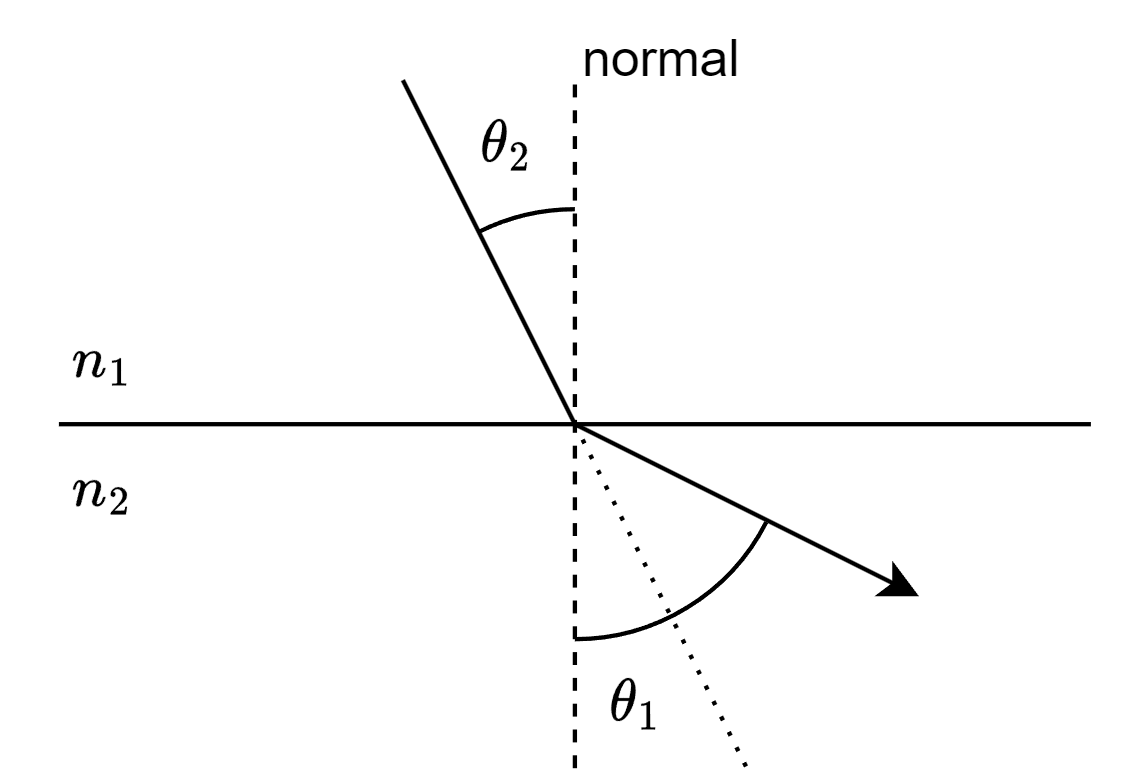
\includegraphics[width=0.5\linewidth]{images/refraction.png}
        \caption{Snell's law}
    \end{figure}
    \begin{definition}
        The \emph{optical axis} is the straight line that connects the center of the two spheres that are used to form the lens. 
    \end{definition}
    The angles of a ray passing through the centers of the spheres can be calculated as follows: 
    \[\alpha_1=\dfrac{y_1}{\rho_1} \:\:\:\:\:\: \alpha_2=-\dfrac{y_2}{\rho_2}\]
    \begin{figure}[H]
        \centering
        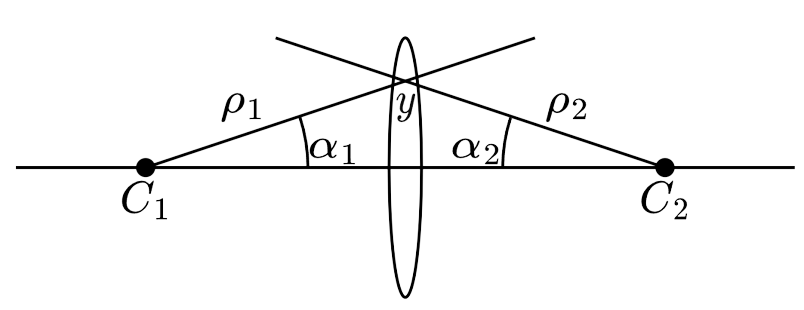
\includegraphics[width=0.5\linewidth]{images/y.png}
    \end{figure}
    Since we have a simplified lens, it is possible to say that:
    \[y_1=y_2=y\]
    
    \section{Light rays deviation}
    \begin{figure}[H]
        \centering
       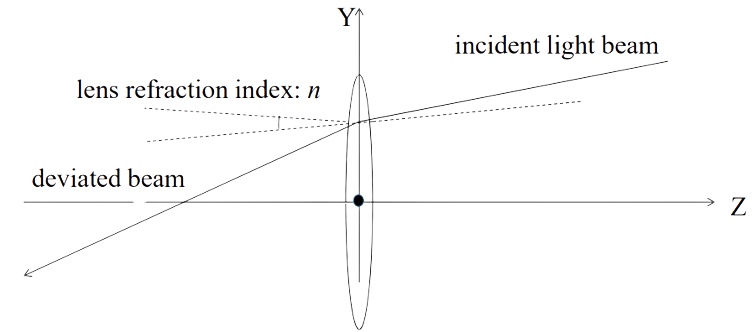
\includegraphics[width=0.5\linewidth]{images/ray.png}
   \end{figure}
    Given a lens with refraction $n$ we have that the following equations are valid:
    \[\dfrac{\theta-\alpha_1}{\theta^{'}-\alpha_1} \Rightarrow \dfrac{\sin{(\theta-\alpha_1)}}{\sin{(\theta^{'}-\alpha_1)}}=n\]
    \[\dfrac{\theta^{''}-\alpha_2}{\theta^{'}-\alpha_2} \Rightarrow \dfrac{\sin{(\theta^{''}-\alpha_2)}}{\sin{(\theta^{'}-\alpha_2)}}=n\]
    where:
    \begin{itemize}
        \item $\theta$ is the angle before the lens. 
        \item $\theta^{'}$ is the angle in the lens (not visible in the image). 
        \item $\theta^{''}$ is the angle after the lens.
    \end{itemize}
    Comparing the two equations it is possible to find the difference between the input angle $\theta$ and the output angle $\theta^{''}$ that is: 
    \[\delta \theta=y(n-1)\left( \dfrac{1}{\rho_1} + \dfrac{1}{\rho_2}\right)\]
    It is possible to see that the first term $(n-1)$ is due to the matter of the lens and the second $\left( \frac{1}{\rho_1} + \frac{1}{\rho_2}\right)$ depend on the curvature 
    of the surface. 

    \section{Focalization of parallel light rays}
    \begin{figure}[H]
        \centering
        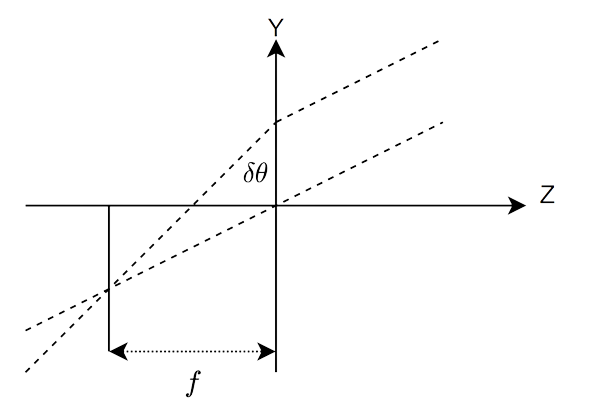
\includegraphics[width=0.5\linewidth]{images/focalization.png}
    \end{figure}
    In the image we have one ray that passes through the center of the lens and the other that passes in another point, but it is parallel to the first one. So we have that: 
    \begin{itemize}
        \item $Y=0$: the deviation of the ray is null and proceed without being deviated. 
        \item $Y=f \cdot \delta \theta \Rightarrow f=\dfrac{1}{(n-1)\left( \dfrac{1}{\rho_1} + \dfrac{1}{\rho_2}\right)}$. 
    \end{itemize}
    This means that all the rays that proceed in parallel meets in one common point on the focal point $Z$, with a distance from the $Y$ axis equal to: 
    \[Z=-f\]

    \section{Path of a light ray}
    To find the projection of a light ray crossing a lens in any position we need to:
    \begin{enumerate}
        \item Draw a line parallel to the selected ray and that passes through the center of the lens. 
        \item Intersect the line with the focal plane.
        \item The ray will go from the point in which it crosses the lens to the point found on the focal plane. 
    \end{enumerate}
    \begin{figure}[H]
        \centering
        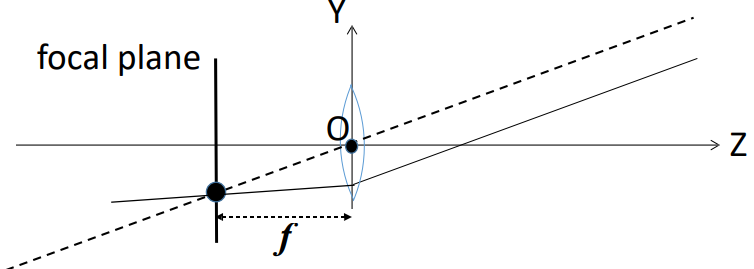
\includegraphics[width=0.5\linewidth]{images/path.png}
        \caption{Path of a light ray through a lens}
    \end{figure}

    \section{Pin-hole camera}
    To have a focussed image we need that every ray hits the focal plane of the camera in exactly one pixel. To obtain this we need that the distance between the lens and
    the source of the ray $Z(P)$ must be much greater than the lens aperture $a$ (at least $1000\times$). In this way we can place the screen at distance $Z$ from the lens. If all they rays
    respect this constraint they will be all parallel for the lens and the image will be on focus. The camera that we have defined so far is called pin-hole camera and needs:
    \begin{enumerate}
        \item Thin spherical lens. 
        \item Small angles.
        \item $Z(P) \gg a$.
        \item $Z=f$.
    \end{enumerate}

    \section{From real world to 2D images}
    The images are in a 2D plane while the real world is in three dimensions. So, a picture have less information than the original subject in the real world. In fact, the space 
    projection of space in a 2D image is a perspective projection, that is: 
    \begin{itemize}
        \item Nonlinear.
        \item Not shape-preserving.
        \item Not length-ratio preserving. 
    \end{itemize}
    Due to the triangle equality we have that:
    \[x=f \dfrac{X}{Z} \:\:\:\:\:\: y=f \dfrac{Y}{Z}\]
    The only way to avoid this information loss is to take a picture of a planar scene on plane parallel to image plane, so we need to have 
    \[Z=Z_0=\textnormal{constant}\]
    \begin{figure}[H]
        \centering
        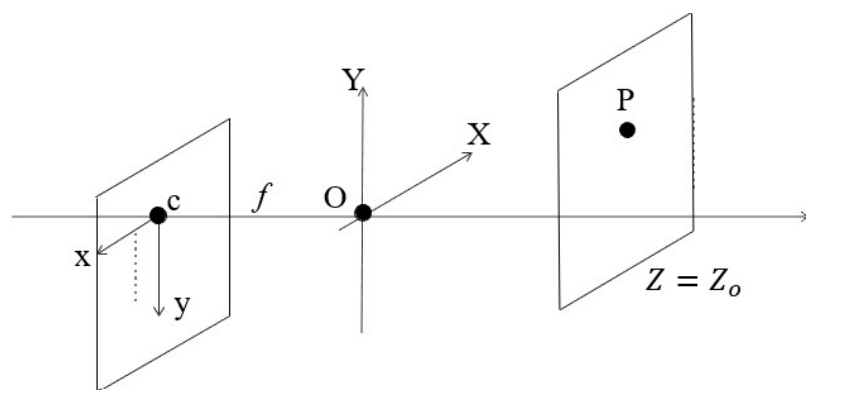
\includegraphics[width=0.5\linewidth]{images/Z0.png}
    \end{figure}
    In this case the only difference between reality and projection will be the down scaling, while the other dimensions are preserved: 
    \[x=f \dfrac{X}{Z_0}=kX \:\:\:\:\:\: y=f \dfrac{Y}{Z_0}=kY \]
    
    \section{Perspective and vanishing point}
    If we decide to choose all the lines parallel to the direction parameters $\begin{bmatrix} \alpha & \beta & 1 \end{bmatrix}$ we obtain the following system: 
    \[
        \begin{cases}
            X = X_0 + \alpha Z  \\
            Y = Y_0 + \beta Z   \\
            Z = 1 \cdot Z
        \end{cases}
    \]
    All these lines can be projected in the 2D image with the triangle equality in the following way: 
    \[x=f \dfrac{X}{Z} = f \dfrac{X_0 + \alpha Z}{Z} = f\alpha + \dfrac{X_0}{Z}\]
    \[y=f \dfrac{Y}{Z} = f \dfrac{Y_0 + \beta Z}{Z}  = f\beta  + \dfrac{Y_0}{Z}\]
    We now want to find the image of the point at the infinity of these lines, so we obtain the point: 
    \[\begin{bmatrix} f\alpha f\beta \end{bmatrix}\]
    that is independent of $X_0$ and $Y_0$. So, we have that all parallel lines have the same image if their points at the infinity.
    \begin{definition}
        The image of the point at the infinity of the lines is called \emph{vanishing point}. 
    \end{definition}
    So, we have that all the lines that are parallel in the real world will project onto concurrent lines in the image. 
    \begin{figure}[H]
        \centering
        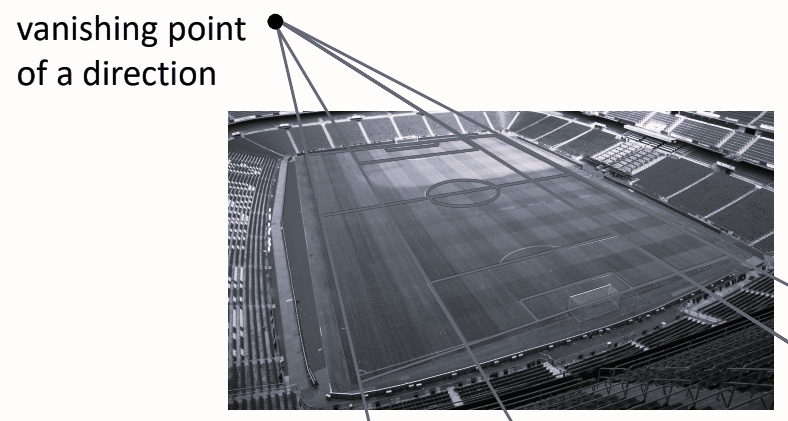
\includegraphics[width=0.75\linewidth]{images/vanishingpoint.png}
        \caption{Example of vanishing point}
    \end{figure}

\newpage

\chapter{Planar Projective Geometry}
    \section{Introduction}
    The elements needed to define a planar geometry are: point, lines, conics and dual conics. The possible transformations in this type of geometry are: projectivities, 
    affinities, similarities and isometries. 

    \section{Points}
    The points can be defined in cartesian coordinates by defining a euclidean plane with his origin. In this way every point is defined unambiguously with two cartesian 
    coordinates $(x,y)$. 

    To analyze images it is better to use homogeneous coordinates. To define this type of coordinates we need to construct a 3D space with $x,y,w$ axis. So, now to define a point
    we have to assign three values. This means that every number can be represented in infinite ways by changing the value of $w$. The correlation between cartesian
    and homogeneous coordinates is the following: 
    \[
    \overline{x} =
    \begin{bmatrix}
        x \\
        y \\
        w 
    \end{bmatrix}
    =w
    \begin{bmatrix}
        X \\
        Y \\
        1 
    \end{bmatrix}
    \]
    So we have that a vector $\overline{x} = \begin{bmatrix} x \\ y \\ w \end{bmatrix}$ and all its nonzero multiples $\lambda \begin{bmatrix} x \\ y \\ w \end{bmatrix}$, including
    $\begin{bmatrix} x/w \\ y/w \\ 1 \end{bmatrix}$, represent the point of cartesian coordinates $\begin{bmatrix} X \\ Y \end{bmatrix}=\begin{bmatrix} x/w \\ y/w\end{bmatrix}$
    on the euclidean plane. This type of representation has the homogeneity property:  any vector $\overline{x}$ is equivalent to all its nonzero multiples $\lambda \overline{x}, 
    \lambda \neq 0$, since they represent the same point. The null vector does not represent any point.
    \begin{definition}
        The \emph{projective plane} is defined as:
        \[\mathbb{P}^2=\{{\begin{bmatrix} x & y & w \end{bmatrix}}^T \in \mathbb{R}^3\}-\{{\begin{bmatrix} 0 & 0 & 0 \end{bmatrix}}^T\}\]
    \end{definition}
    \begin{example}
        The origin of the plane is defined as:
        \[{\begin{bmatrix} 0 & 0 & 1 \end{bmatrix}}^T\]
        A generic point in heterogeneous coordinates can be transformed into a couple of cartesian coordinate with a simple division. The point:
        \[{\begin{bmatrix} 0 & 8 & 4 \end{bmatrix}}^T\]
        in cartesian coordinate is equal to: 
        \[{\begin{bmatrix} x/w & y/w  \end{bmatrix}}^T=\begin{bmatrix} 0/4 & 8/4 \end{bmatrix}=\begin{bmatrix} 0 & 4 \end{bmatrix}\]
    \end{example}
    Consider the point $\overline{x}=\begin{bmatrix} x \\ y \\ w \end{bmatrix}$ and let $w$ slowly drop to $0$ starting from $w=1$. As $w$ decreases, the point will move along a 
    constant direction $\begin{bmatrix} x & y \end{bmatrix}$, with increasing distance from the origin. As $w$ tends to $0$, this points tends to the infinity along the direction 
    $\begin{bmatrix} x & y \end{bmatrix}$. 
    \begin{definition}
        The point \[\overline{x} = \begin{bmatrix} x \\ y \\ w \end{bmatrix}\] is called the \emph{point at the infinity along the direction} $\begin{bmatrix} x & y \end{bmatrix}$. 
    \end{definition}
    Points at the infinity, who represent directions, are not part of the euclidean plane: they are extra points, well-defined within the projective plane. So, in general we have
    that the projective plane is the euclidean plane with also the points at the infinity. 

    \section{Lines}
    In the euclidean plane a line is defined as: 
    \[aX+bY+c=0\]
    In the heterogeneous plane the lines are defined as: 
    \[a\dfrac{x}{w}+b \dfrac{y}{w}+c=0 \Longrightarrow ax+by+cw=0\]
    This equation can be also represented using two vectors called respectively $\overline{l}^T$ and $\overline{x}$:
    \[\begin{bmatrix} a & b & c \end{bmatrix} \begin{bmatrix} x \\ y \\ w \end{bmatrix}=0\]
    where the vector $\overline{l}={\begin{bmatrix} a & b & c \end{bmatrix}}^T$ and all its nonzero multiples represent a line. This type of representation has the homogeneity
    property: any vector $\overline{l}$ is equivalent to all its nonzero multiples $\lambda \overline{l}, \lambda \neq 0$, since they represent the same line. $a,b,c$ are called 
    homogeneous parameters of the line. 

    As for numbers, there is an infinite number of equivalent representations for a single line, namely all nonzero multiples of the unit normal vector. The null vector does not
    represent any lines.
    \begin{definition}
        The \emph{projective dual plane} is defined as: 
        \[\mathbb{P}^2=\{{\begin{bmatrix} a & b & c \end{bmatrix}}^T \in \mathbb{R}^3\}-\{{\begin{bmatrix} 0 & 0 & 0 \end{bmatrix}}^T\}\]
    \end{definition}

    There are three important remarks: 
    \begin{enumerate}
        \item If the third parameter is null, ${\overline{l}=\begin{bmatrix} a & b & 0 \end{bmatrix}}^T$, then the line goes through point $\begin{bmatrix} 0 & 0 \end{bmatrix}$. 
        \item Within the euclidean plane, direction $\begin{bmatrix} a & b \end{bmatrix}$ is normal to the line \\ ${\overline{l}=\begin{bmatrix} a & b & c \end{bmatrix}}^T$. 
        \item Two lines ${\overline{l}=\begin{bmatrix} a & b & c \end{bmatrix}}^T$ and ${\overline{l}=\begin{bmatrix} a & b & c^{'} \end{bmatrix}}^T$ are parallel: their common 
            direction is $[b,-a]$. 
    \end{enumerate}
    \begin{example}
        The cartesian axes are defined as: 
        \[\overline{l}_x=\begin{bmatrix} 0 \\ 1 \\ 0 \end{bmatrix} \:\:\:\:\:\: \overline{l}_y=\begin{bmatrix} 1 \\ 0 \\ 0 \end{bmatrix}\]
    \end{example}
    The incidence relation of a line $\overline{l}^T\overline{x}=0$ is defined when: 
    \begin{itemize}
        \item The point $\overline{x}$ is on the line $\overline{l}$ or
        \item The line $\overline{l}$ goes through the point $\overline{x}$. 
    \end{itemize}
    \begin{definition}
        The line \[\begin{bmatrix} 0 & 0 & 1 \end{bmatrix} \begin{bmatrix} x \\ y \\ w \end{bmatrix}=\overline{w}=0\] is called the \emph{line at the infinity} $\overline{l}_{\infty}={\begin{bmatrix} 0 & 0 & 1 \end{bmatrix}}^T$. 
    \end{definition}
    Since the dot product is commutative, also the incidence relation is commutative, so the sentences "point $\overline{x}$ is on line $\overline{l}$" and "point $\overline{l}$ is 
    on line $\overline{x}$" have the same algebraic meanings. This is called the principle of duality between points and lines. 
    Given the lines $\overline{l}_1^T$ and $\overline{l}_2^T$, the intersection can be found by imposing: 
    \[\begin{bmatrix} \overline{l}_1^T \\ \overline{l}_2^T \end{bmatrix} \overline{x} = \begin{bmatrix} 0 \\ 0 \end{bmatrix}\]
    that is equal to find the right null space of the first column vector. 
    \[\overline{x}=\textbf{RNS}\left( \begin{bmatrix} \overline{l}_1^T \\ \overline{l}_2^T \end{bmatrix} \right)\]
    The system found is underdetermined, so there is only one intersection point between two lines (that can be represented in infinite ways in homogeneous plane). Note that the 
    vector $\overline{x}$ is orthogonal to both lines, so in the 2D projective geometry can be found with the cross product: 
    \[\overline{x}=\overline{l}_1 \times \overline{l}_2\]
    \begin{example}
        Suppose we have two parallel lines $\overline{l}_1={\begin{bmatrix} a & b & c_1 \end{bmatrix}}^T$ and 
        $\overline{l}_2={\begin{bmatrix} a & b & c_2 \end{bmatrix}}^T$. The point that is common to both points can be found with the system: 
        \[
            \begin{cases}
                ax+by+c_1w=0 \\
                ax+by+c_2w=0
            \end{cases}
        \]
        So the solution will be ${\overline{x}=\begin{bmatrix} b & -a & 0 \end{bmatrix}}^T$ that is the point at the infinity along the direction of both lines. 
    \end{example}
    The line through two points can be found with the dual of the previous problem, that is: 
    \[\begin{bmatrix} \overline{x}_1^T \\ \overline{x}_2^T \end{bmatrix} \overline{l} = \begin{bmatrix} 0 \\ 0 \end{bmatrix}\]
    that in 2D become: 
    \[\overline{l}=\overline{x}_1 \times \overline {x}_2\] 
    \begin{example}[Property]
        The point $\overline{x}$ given by the linear combination $\overline{x}=\alpha\overline{x}_1+\beta\overline{x}_2$ of two points $\overline{x}_1$ and $\overline{x}_2$ is on the 
        line $\overline{l}$ through $\overline{x}_1$ and $\overline{x}_2$. 
    \end{example}
    \begin{proof}
        The line $\overline{l}$ through both points satisfies $\overline{l}^T\overline{x}_1=0$ and  $\overline{l}^T\overline{x}_2=0$. By adding $\alpha$ times the first 
        equation to $\beta$ times the second one, we obtain: 
        \[0=\overline{l}^T\left( \alpha\overline{x}_1+\beta\overline{x}_2 \right)=\overline{l}^T\overline{x}=0\]
    \end{proof}
    This proves that there is also a duality between colinear and concurrent. 
    \begin{theorem}[duality principle]
        For any true sentence containing the words: point, line, is on and goes through there is a dual sentence (also true) obtained by substituting, in the previous one, each 
        occurrence of: 
        \begin{itemize}
            \item Point $\Leftrightarrow$ line. 
            \item Is on $\Leftrightarrow$ goes through.
            \item Colinear $\Leftrightarrow$ concurrent. 
        \end{itemize}
    \end{theorem}
    Within the euclidean plane, $\begin{bmatrix} a & b \end{bmatrix}$ is the direction normal to the line $\overline{l}={\begin{bmatrix} a & b & c \end{bmatrix}}^T$. Since we have that
    the angle between two lines is the angle between their normal and that the angle between two vectors is equal to:
    \[\cos\theta=\dfrac{\overline{u} \cdot \overline{v}}{\left\lvert \overline{u} \right\rvert \left\lvert \overline{v} \right\rvert}\] 
    we have that the angle between two lines $\overline{l}_1={\begin{bmatrix} a_1 & b_1 & c_1 \end{bmatrix}}^T$ and $\overline{l}_2={\begin{bmatrix} a_2 & b_2 & c_2 \end{bmatrix}}^T$ 
    is the angle between their normal directions $\begin{bmatrix} a_1 & b_1 \end{bmatrix}$ and $\begin{bmatrix} a_2 & b_2 \end{bmatrix}$, namely: 
    \[\cos\theta=\dfrac{a_1a_2+b_1b_2}{\sqrt{\left( a_1^2 + b_1^2 \right)\left( a_2^2 + b_2^2 \right)}}\]
    
    The ratio of length is an invariant.

    Given a line with four points that have the following relations: 
    \[\overline{X}_1=\alpha_1\overline{Y}+\beta_1\overline{Z}\]
    \[\overline{X}_2=\alpha_2\overline{Y}+\beta_2\overline{Z}\]
    We have that the cross ratio is the following: 
    \[CR_{X_1,X_2,Y,Z}=\dfrac{c-a}{c-b}/\dfrac{d-a}{d-b}=\dfrac{\beta_1/\alpha_1}{\beta_2/\alpha_2}\]
    \begin{figure}[H]
        \centering
        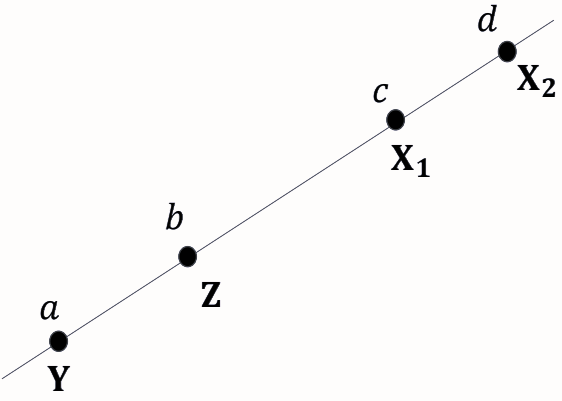
\includegraphics[width=0.25\linewidth]{images/line.png}
        \caption{Line with the point of previous problem}
    \end{figure}
    \begin{proof}
        Since the abscissae are proportional we can replace the abscissae by the $X$ coordinate like in the figure. 
        \begin{figure}[H]
            \centering
            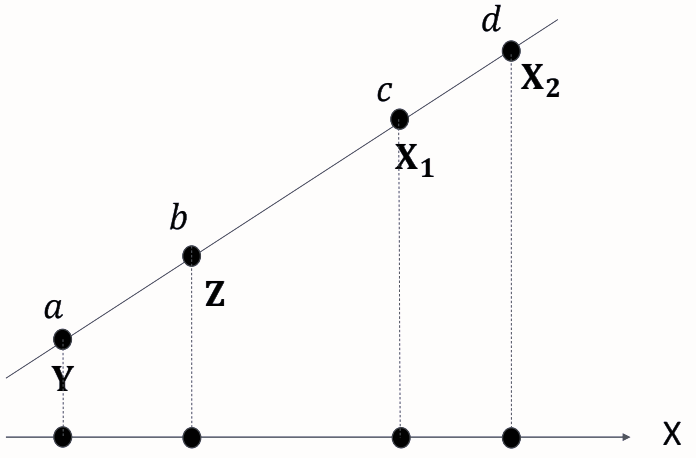
\includegraphics[width=0.4\linewidth]{images/abscissae.png}
        \end{figure}
        And the relation 
        \[CR_{X_1,X_2,Y,Z}=\dfrac{c-a}{c-b}/\dfrac{d-a}{d-b}\]
        still holds. Let $\overline{Y}=\begin{bmatrix} y \\ * \\ v \end{bmatrix}$ and $\overline{Z}=\begin{bmatrix} z \\ * \\ w \end{bmatrix}$, then: 
        \[ \overline{X}_1=\begin{bmatrix} \alpha_1y+\beta_1z \\ * \\ \alpha_1v+\beta_1w \end{bmatrix} \:\:\:\:\:\:\:\:\:\:\:\:
        \overline{X}_2=\begin{bmatrix} \alpha_2y+\beta_2z \\ * \\ \alpha_2v+\beta_2w \end{bmatrix}\]
        The difference between the $X$ coordinates of $\overline{X}_1$ and $Y$ is:
        \[c-a=\dfrac{\beta_1(zv-yw)}{(\alpha_1y+\beta_1z)v}\]
        The difference between the $X$ coordinates of $\overline{X}_1$ and $Z$ is:
        \[c-b=\dfrac{-\alpha_1(zv-yw)}{(\alpha_1y+\beta_1z)w}\]
        By substitution we obtain: 
        \[ \dfrac{c-a}{c-b}=-\dfrac{\beta_1w}{\alpha_1v} \:\:\:\:\:\:\:\:\:\:\:\: \dfrac{d-a}{d-b}=-\dfrac{\beta_2w}{\alpha_2v}\]
    \end{proof}

    \section{Conics}
    The conics derives from the intersection of cones with planes. 
    \begin{figure}[H]
        \centering
        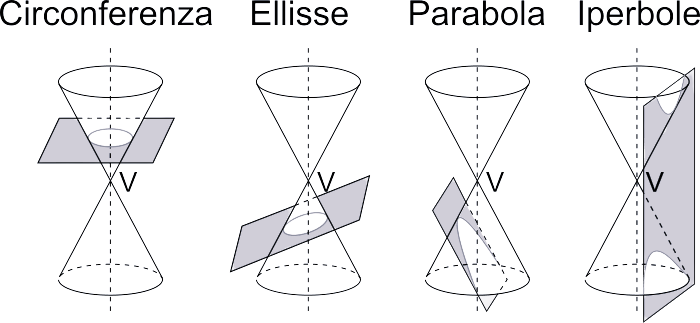
\includegraphics[width=0.75\linewidth]{images/conics.png}
        \caption{Conics}
    \end{figure}
    \begin{definition}
        A point $\overline{x}$ is on a \emph{conic} $\overline{C}$ if it satisfies a homogeneous quadratic equation, namely
        \[\overline{x}^T\overline{C}\overline{x}=0\]
        where $\overline{C}$ is a symmetric matrix (this is a convention). 
    \end{definition}
    A conic is a curve described by a second-degree equation in the plane. In Euclidean coordinates a conic becomes: 
    \[aX^2+bXY+cY^2+dX+eY+f=0\]
    and in homogeneous coordinates becomes: 
    \[ax^2+bxy+cy^2+dxw+eyw+fw^2=0\]
    or in matrix form: 
    \[\overline{x}^T \begin{bmatrix} a & b/2 & d/2 \\ b/2 & c & e/2 \\ d/2 & e/2 & f \end{bmatrix} \overline{x}=0\]
    The conics have five degrees of freedom, so we need five points to define a unique conic. 
    \begin{example}
        The circumference can be expressed in cartesian coordinates: 
        \[(X-X_0)^2+(Y-Y_0)^2-r^2=0\]
        or in homogeneous coordinates: 
        \[  \begin{bmatrix} x & y & w \end{bmatrix}
            \begin{bmatrix} 1 & 0 & -X_0 \\ 0 & 1 & -Y_0 \\ -X_0 & -Y_0 & X_0^2+Y_0^2-r^2 \end{bmatrix}
            \begin{bmatrix} x \\ y \\ w \end{bmatrix} = 0
        \]
    \end{example}
    Given a quadratic equation of a conic and a linear equation of a line, their intersection leads to a two degree equation on $\overline{x}$. This means that there are always two 
    intersection points between a line and a conic, and they can be: real or complex conjugate and distinct or coincident. This result is due to the fundamental theorem of algebra. 
    \begin{theorem}[Fundamental theorem of algebra]
        The fundamental theorem of algebra states that every non-constant single-variable polynomial with complex coefficients has at least one complex root.
    \end{theorem}
    \begin{figure}[H]
        \centering
        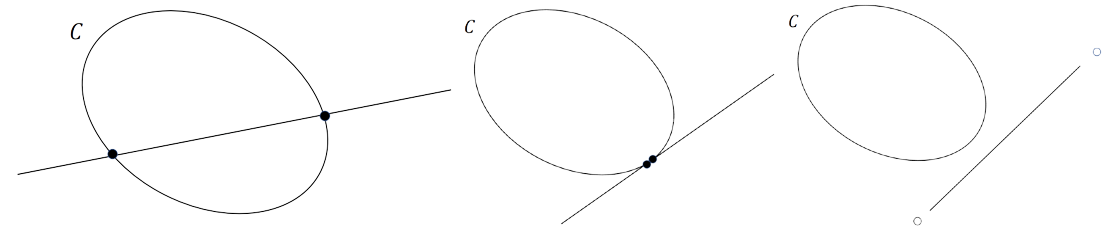
\includegraphics[width=0.75\linewidth]{images/intersection.png}
        \caption{Intersection with two real roots, two coincident roots and two imaginary roots}
    \end{figure}


\end{document}